\section{基于Boosting的集成}
\label{sec:ensemble-boosting}

把许多相近成员平均，只能抵消成员特有的波动，无法补上所有成员共同遗漏的结构。Boosting换一种顺序：先看当前组合在哪些记录上系统性地没学好，再让新成员专门去补这一部分，逐轮把欠拟合的结构加上。各轮成员依次依赖前面的组合，但同一轮内部的候选拟合仍是独立计算。下面先给出所有Boosting方法共享的加法模型与前向逐步框架，再分别讲AdaBoost、GBDT、LogitBoost、XGBoost、LightGBM与CatBoost；注意区分“损失准则”与“训练机制”，前者决定补什么，后者决定怎样搜索。

\subsection{共同模型与前向逐步学习}
\label{sec:ensemble-stagewise-additive}

\subsubsection{模型结构}
Boosting把预测写成成员的加法组合
\begin{equation}
  F_M(\bm x)=F_0(\bm x)+\sum_{t=1}^M f_t(\bm x),
  \label{eq:ensemble-additive}
\end{equation}
其中$F_0$是初始值（回归常取训练均值，分类常取先验对数几率），每个$f_t$属于预先选定的成员族（树、线性修正等），最终输出按任务转换为数值、类别或概率。这里待学的正是逐轮加入的成员$f_t$及其组合系数；$F_0$只按训练数据初始化，此后固定，不逐轮调整。

\subsubsection{参数学习}

前向逐步学习在第$t$轮固定已有组合$F_{t-1}$，只选择本轮成员$f_t$及其系数，使本轮目标最小：
\begin{equation}
  f_t,\beta_t=\arg\min_{f,\beta}\sum_{i=1}^n L\big(y_i,\,F_{t-1}(\bm x_i)+\beta f(\bm x_i)\big)+\Omega(f),
  \label{eq:ensemble-stagewise}
\end{equation}
其中$L$是任务损失，$\Omega$是成员复杂度惩罚。旧成员的参数在本轮不再调整。成员族、损失与待估未知量三者由任务确定：平方损失配回归树，指数损失配分类成员，对数损失配概率输出。

无约束时惩罚项为零；采用回归树作为成员时，惩罚通常包含叶数与叶值平方两部分，并要求组合系数非负。惩罚施加在本轮实际加入的函数$\beta f$上，而不是孤立地惩罚成员$f$。这里存在缩放关系：若把成员参数整体放大$c$倍、把系数缩小$c$倍，$\beta f$不变但叶值平方罚的计算口径会改变，因此要明确罚的是哪一个。

式\eqref{eq:ensemble-stagewise}直接优化的是实际增量$\beta f$；另一种常见实现先拟合一个未收缩的成员$f_t^{\mathrm{raw}}$，再乘以学习率$\nu\in(0,1]$加入组合，即$F_t=F_{t-1}+\nu f_t^{\mathrm{raw}}$。后者不再严格最小化同一代理目标，$\nu$是额外的保守步幅，不能把收缩后的叶值仍称作该代理目标的精确最优。

前向逐步每轮只在当前候选族内比较，得到的是逐步贪心解，不是全体成员联合优化的全局最优。梯度与牛顿的一般原理参考卷一，各模型从自身目标推出修正方向、成员拟合与更新规则，本地完成推导。

\subsection{AdaBoost}
\label{sec:ensemble-adaboost}

所有样本同权训练时，已经分对的记录反复参与，难分记录始终占同样份量，新成员继续学不好它们。AdaBoost让每轮训练都提高上一轮错分记录的份量，并按成员的好坏分配它在投票中的发言权。

\subsubsection{模型结构}
二分类标签取$y_i\in\{-1,+1\}$，弱成员$h_t(\bm x)\in\{-1,+1\}$（只比随机猜测略好、错误率略低于$1/2$的成员）给出判断，加法得分与决策为
\begin{equation}
  F_T(\bm x)=\sum_{t=1}^T\alpha_t h_t(\bm x),
  \qquad
  \hat y(\bm x)=\operatorname{sign}(F_T(\bm x)),
  \label{eq:ensemble-adaboost-model}
\end{equation}
$\alpha_t>0$是成员投票系数，平局规则事先固定。

\subsubsection{参数学习}

\paragraph{成员训练与投票系数}
第$t$轮样本权重归一化后为$w_i^{(t)}$，成员在加权样本上训练，加权错误率为
\begin{equation}
  \epsilon_t=\sum_{i:h_t(\bm x_i)\neq y_i}w_i^{(t)}.
  \label{eq:ensemble-adaboost-error}
\end{equation}
AdaBoost对应指数损失$L(y,F)=e^{-yF}$（打分离真实标签越远，惩罚指数级增长）。在已有得分$F_{t-1}$上加入$\alpha h_t$后，本轮要最小化的归一化指数加权和为
\[
  Z_t(\alpha)=\sum_i w_i^{(t)}e^{-\alpha y_i h_t(\bm x_i)}
  =e^{-\alpha}\sum_{\text{分对}}w_i^{(t)}+e^{\alpha}\sum_{\text{错分}}w_i^{(t)}
  =e^{-\alpha}(1-\epsilon_t)+e^{\alpha}\epsilon_t,
\]
其中$\sum_{\text{错分}}w_i^{(t)}=\epsilon_t$是错分样本的权重和，$\sum_{\text{分对}}w_i^{(t)}=1-\epsilon_t$。对$\alpha$求导并令其为零：$-(1-\epsilon_t)e^{-\alpha}+\epsilon_t e^{\alpha}=0$，整理得$e^{2\alpha}=(1-\epsilon_t)/\epsilon_t$，即投票系数
\begin{equation}
  \alpha_t=\frac12\ln\frac{1-\epsilon_t}{\epsilon_t}.
  \label{eq:ensemble-adaboost-alpha}
\end{equation}

\paragraph{样本权重与停止规则}
更新后的样本权重归一化为
\begin{equation}
  w_i^{(t+1)}=\frac{w_i^{(t)}\exp[-\alpha_t y_i h_t(\bm x_i)]}{Z_t},
  \qquad
  Z_t=\sum_i w_i^{(t)}\exp[-\alpha_t y_i h_t(\bm x_i)].
  \label{eq:ensemble-adaboost-update}
\end{equation}
分对样本乘$e^{-\alpha_t}$、错分样本乘$e^{\alpha_t}$，相对变化由此可见。例如$\epsilon_t=1/4$时$\alpha_t=\frac12\ln3\approx0.549$，错分样本权重约为分对样本的$e^{2\alpha_t}=3$倍。若$\epsilon_t=0$，当前成员已分对全部加权样本，直接输出$h_t$并停止，避免代入发散系数（参考\BookChapterRef{chap:binary-learnability}{卷三《基础、理论与可信性》“二分类学习的可学习性”章}）。正投票系数要求$\epsilon_t<1/2$；条件未满足时可停止本轮、调整训练或采用相应变体。持续被错分的噪声标签（标签本身标错的样本）会获得越来越大的权重，需要在数据层面处理。整轮流程是“加权重训弱成员、按加权错误率解析确定投票系数”，并不是直接对投票系数做梯度下降。

\begin{figure*}[htbp]
  \centering
  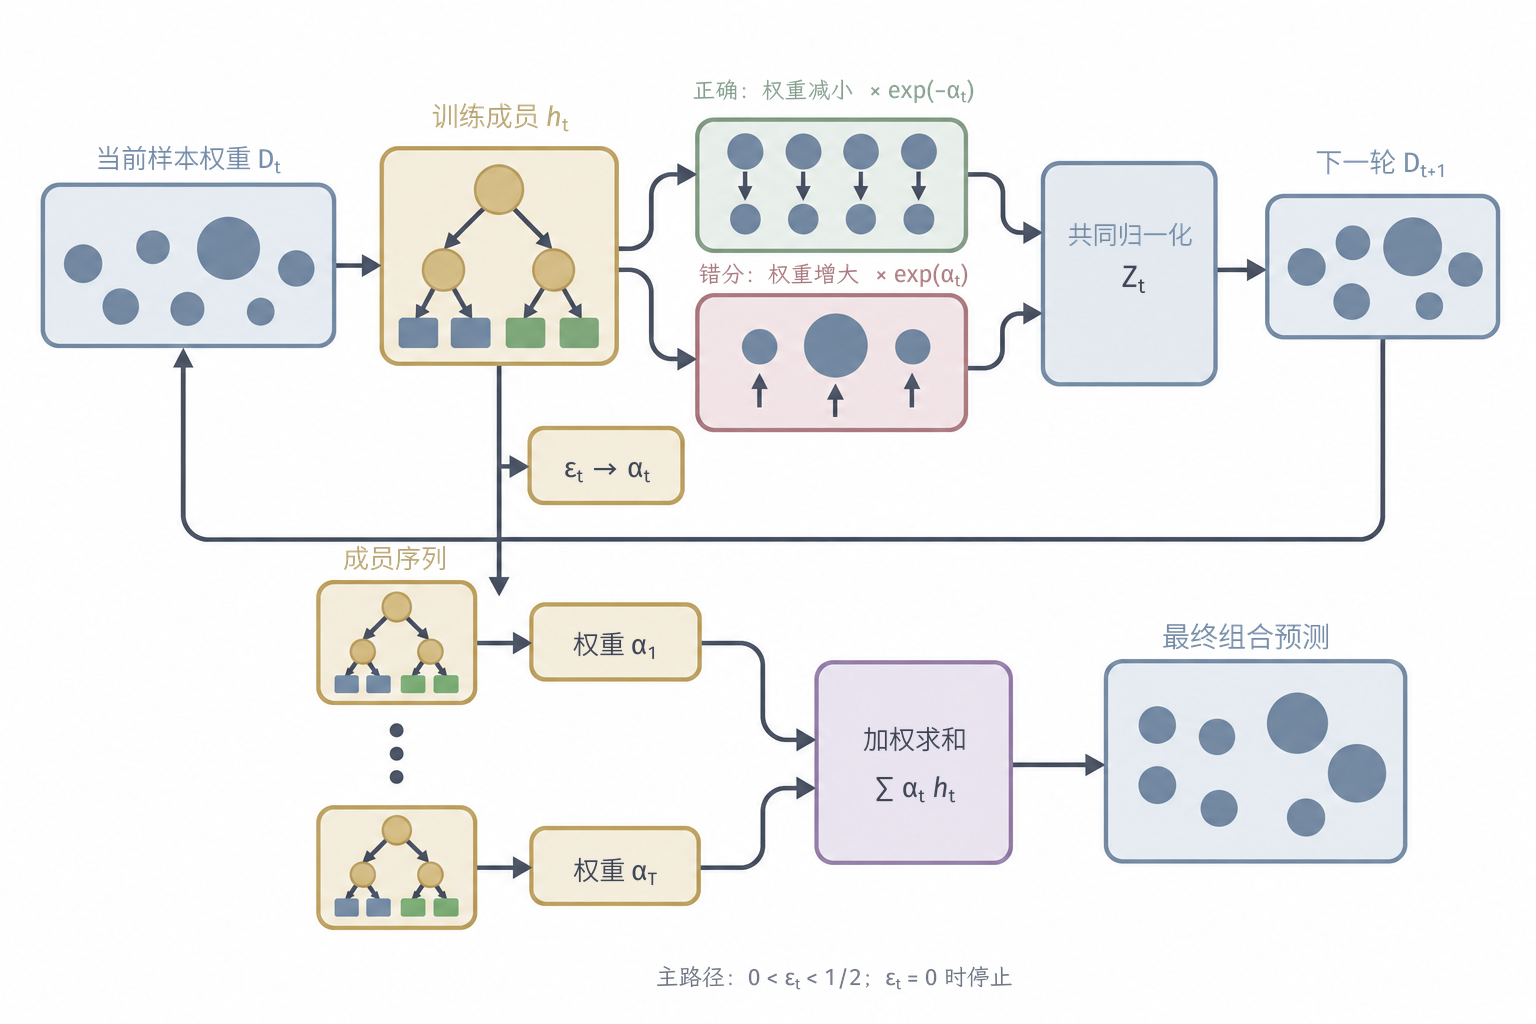
\includegraphics[width=130.048mm]{figures/07-classic-models/00-shared/generated/ensemble-adaboost-weight-update/figure.png}
  \caption{AdaBoost样本权重更新示意：错分样本权重上升、分对样本权重下降（教学构造）。}
  \label{fig:ensemble-adaboost-weight-update}
\end{figure*}

\subsubsection{理论分析}
\label{sec:ensemble-adaboost-theory}
指数损失满足$1[\operatorname{sign}F(\bm x_i)\neq y_i]\le e^{-y_iF(\bm x_i)}$，因此训练错误率被平均指数损失$\frac1n\sum_i e^{-y_iF_T(\bm x_i)}$上界控制。再把这个平均指数损失用权重递推显式展开：把$w_i^{(t+1)}=w_i^{(t)}e^{-\alpha_t y_i h_t(\bm x_i)}/Z_t$逐轮代入，得$w_i^{(T+1)}=w_i^{(0)}\prod_{t=1}^T e^{-\alpha_t y_i h_t(\bm x_i)}/Z_t$；取初始权重$w_i^{(0)}=1/n$、加法模型$F_T=\sum_t\alpha_t h_t(\bm x_i)$，则$w_i^{(T+1)}=\frac1n e^{-y_iF_T(\bm x_i)}\big/\prod_{t=1}^T Z_t$。两边同乘$\prod_{t=1}^T Z_t$并对$i$求和，由归一化$\sum_iw_i^{(T+1)}=1$，平均指数损失恰等于连乘$\prod_{t=1}^T Z_t$。每轮$Z_t$在上述最优$\alpha_t$处取最小值$2\sqrt{\epsilon_t(1-\epsilon_t)}$；记弱优势$\gamma_t=1/2-\epsilon_t$，则$2\sqrt{\epsilon_t(1-\epsilon_t)}=2\sqrt{1/4-\gamma_t^2}\le e^{-2\gamma_t^2}$，于是训练错误率满足
\begin{equation}
  \frac1n\sum_i\mathbf1[\hat y(\bm x_i)\neq y_i]
  \le \prod_{t=1}^T Z_t
  \le \exp\!\left(-2\sum_{t=1}^T\gamma_t^2\right).
  \label{eq:ensemble-adaboost-bound}
\end{equation}

只有当每轮$\gamma_t>0$（弱成员好于随机猜测）时连乘因子才小于$1$；若$\gamma_t$有一致的正下界，训练错误率按指数衰减。$\epsilon_t=0$的可分情形由停止规则处理，不代入发散系数。该界只约束训练样本上的错误率，不假设样本独立或成员复杂度条件，因而不构成对新样本的保证；持续错分的噪声标签会被逐轮放大权重。

\subsubsection{多分类AdaBoost：SAMME}
\label{sec:ensemble-adaboost-multiclass}
二分类符号规则不能直接用于$K>2$类：\term{SAMME}（Stagewise Additive Modeling using a Multiclass Exponential loss function）改为对每一类分别累计成员投票，$h_t^{(c)}(\bm x)\in\{0,1\}$为第$t$个成员把输入判给类$c$的指示，最终按各类得分$\sum_t\alpha_t h_t^{(c)}(\bm x)$取最大类决策；投票系数修正为
\begin{equation}
  \alpha_t=\frac12\ln\frac{1-\epsilon_t}{\epsilon_t}+\ln(K-1),
  \label{eq:ensemble-samme-alpha}
\end{equation}
其中$\epsilon_t$为多分类加权错误率。额外的$\ln(K-1)$项补偿随机猜测的基准概率$1/K$：只有当加权错误率低于$1-1/K$时$\alpha_t$才为正。成员在加权多分类样本上训练，样本权重更新形式与式\eqref{eq:ensemble-adaboost-update}相同\scite{zhu2009samme}。

\subsection{梯度提升机与GBDT}
\label{sec:ensemble-gradient-boosting}

固定当前组合后，要为每一条记录定出下一轮该往哪个方向修正、修多少；损失对当前预测的导数正好给出这个方向，把逐点方向拟合成树，新成员就成了可用于新输入的修正。

\subsubsection{模型结构}
\term{梯度提升机}（gradient boosting machine, GBM）以连续加法模型$F_M(\bm x)=F_0+\sum_t f_t(\bm x)$为框架；成员取叶常数回归树时称为\term{梯度提升决策树}（gradient boosted decision tree, GBDT）。同一叶内的样本共享同一个修正值，叶值是该区域的集体修正，不是为单个预测点自由拟合的参数；最终输出经任务链接转为分类概率或回归数值。

\subsubsection{参数学习}

\paragraph{负梯度与方向拟合}
对可微损失$L(y,F)$，第$t$轮在当前组合$F_{t-1}$处的负梯度为
\begin{equation}
  r_{ti}=-\left[\frac{\partial L(y_i,F)}{\partial F}\right]_{F=F_{t-1}(\bm x_i)},
  \label{eq:ensemble-pseudo-residual}
\end{equation}
平方损失$L=\frac12(y-F)^2$对当前得分的导数为$\partial L/\partial F=F-y$，取负即$r_{ti}=y_i-F_{t-1}(\bm x_i)$，恰好是普通残差。回归树以平方误差拟合这组负梯度，得到叶区域$R_{tj}$与叶均值；有限样本下$F_0$取使初始损失最小的常数（平方损失取训练均值）。图\ref{fig:ensemble-boosting-residuals}展示平方损失下的一次更新：新成员拟合的是残差，再把输出加回已有预测，偏高的预测随负残差降低、偏低的随正残差升高。拟合目标是负梯度方向，不是直接拟合原始标签；这一区分在换损失时尤其重要。

\begin{figure*}[tbp]
  \centering
  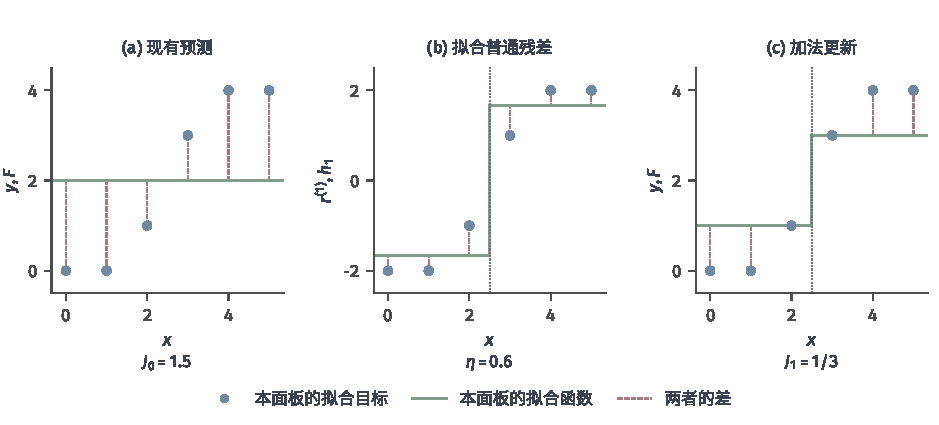
\includegraphics[width=159.000mm]{figures/07-classic-models/00-shared/matplotlib/ensemble-boosting-residuals/figure.pdf}
  \caption{平方损失下的一次梯度提升更新。六个输入为$x=0,\ldots,5$，响应依次为$0,0,1,3,4,4$，常数初始化$F_0=2$。在相邻输入中点中搜索，最小二乘残差树选取阈值$2.5$，两叶输出分别为$-5/3$与$5/3$。取$\eta=0.6$，$F_1=F_0+\eta h_1$在两侧分别为$1$与$3$；平均损失$J_t=(2n)^{-1}\sum_i[y_i-F_t(x_i)]^2$由$1.5$降至$1/3$。蓝点依次表示观测、残差、观测，绿线为各面板的拟合函数，红色虚线为两者之差。数据与更新均为可复核的教学构造，这个普通残差计算依赖平方损失。}
  \label{fig:ensemble-boosting-residuals}
\end{figure*}

\paragraph{步幅与模型更新}
对每个叶区域沿该方向搜索最优步幅
\[
  \rho_{tj}=\arg\min_{\rho}\sum_{\bm x_i\in R_{tj}}L\bigl(y_i,F_{t-1}(\bm x_i)+\rho\bigr),
\]
再更新
\begin{equation}
  F_t(\bm x)=F_{t-1}(\bm x)+\sum_j\rho_{tj}\mathbf1[\bm x\in R_{tj}].
  \label{eq:ensemble-gbdt-update}
\end{equation}
逐叶线搜索与单一全局步幅是两种实现，更新形式不同，不要混为一谈。

\paragraph{不同损失及后续调整}
平方损失关注条件均值；二项对数损失$L=-[y\log p+(1-y)\log(1-p)]$在$p=\sigma(F)$时的导数为$\partial L/\partial F=p-y$，取负得伪响应$r_{ti}=y_i-p_i$（$p_i$为当前概率），叶值修正概率对数几率而非概率本身，不能把实数值修正直接加到概率上。在此基础上，收缩改变增量幅度、随机采样改变本轮样本、DART改变参照的已有组合、分位数提升改变预测目标，分别在下面几小节展开。

\subsubsection{收缩与早停：控制累积拟合}
\label{sec:ensemble-shrinkage}

\paragraph{收缩系数与累积模型}
\term{收缩}（shrinkage）以$\nu\in(0,1]$缩放每轮增量：$F_t=F_{t-1}+\nu\sum_j\rho_{tj}\mathbf1[\bm x\in R_{tj}]$。它减慢累积拟合，降低单轮过大修正的影响；$\nu$越小需要的轮数通常越多，与成员复杂度在同一验证口径下联合选择。

\paragraph{验证轨迹与早停}
在独立验证集上逐轮记录损失，损失连续若干轮不再下降时停止，以验证轨迹确定轮数；早停轮数本身使用了验证信息，最终评价仍需另一份未参与选择的数据。

\subsubsection{随机梯度提升：改变本轮样本}
\label{sec:ensemble-stochastic-gb}
\term{随机梯度提升}（stochastic gradient boosting）每轮按比例对记录自助或无放回采样，只在采样子集上计算负梯度并拟合成员\scite{friedman2002stochastic}。采样既增加成员多样性，也降低单轮计算量；采样比例与轮数、收缩一起配置。

\subsubsection{DART：改变本轮参照的已有组合}
\label{sec:ensemble-dart}
普通GBDT在后期参照完整的已有组合拟合负梯度，新增树容易被前面树的贡献掩盖。\term{DART}（Dropout Additive Regression Trees）在计算本轮负梯度前随机丢弃若干已有树，使本轮参照的组合暂时变小，新树被迫补回被丢弃部分；加回时按丢弃比例缩放以保持整体贡献规模\scite{rashmi2015dart}。它改变的是本轮参照的已有组合，不是本轮样本。

\subsubsection{分位数提升：改变预测目标}
\term{分位数提升}（quantile boosting）把第\ref{sec:regression-quantiles}节的分位数损失$\ell(y,z)=\rho_\tau(y-z)$用于提升，成员学习减少该分位目标的偏差。损失在$z=y$处不可微，修正信号改用负次梯度（损失在尖点不可微时，夹在左右斜率之间的一个可行下降方向），例如约定
\[
  r_{ti}=\begin{cases}\tau-1,&y_i<F_{t-1}(\bm x_i),\\ \tau,&y_i\ge F_{t-1}(\bm x_i).\end{cases}
\]
平方损失得到条件均值，分位数损失得到条件分位点，预测目标不同，成员修正的对象随之改变。

\subsection{LogitBoost}
\label{sec:ensemble-logitboost}

指数损失只管把分类推对，输出却不是概率。需要逐轮加法地把事件概率直接学出来时，把AdaBoost的序贯加法框架换成二项对数损失；它与AdaBoost共享加法结构，损失和修正信号都不同，所以单独展开，不附在指数损失算法后面。

\subsubsection{模型结构}
标签以$y_i\in\{0,1\}$编码，模型对完整logit做加法拟合，经Sigmoid转概率：
\begin{equation}
  p(\bm x)=\sigma(F(\bm x))=\frac{1}{1+e^{-F(\bm x)}},
  \qquad
  F_M(\bm x)=F_0(\bm x)+\sum_t f_t(\bm x).
  \label{eq:ensemble-logitboost-model}
\end{equation}
初始$F_0$取先验对数几率，成员为实数值修正，最终按阈值决策；不要在完整logit与概率之间来回切换。

\subsubsection{参数学习}

\paragraph{二阶目标与工作响应}
二项对数损失在当前概率$p_i$处的一阶导为$p_i-y_i$，曲率$v_i=p_i(1-p_i)$（损失对得分的二阶导，反映该点附近曲线弯得多厉害，用于估计一步能迈多大），工作响应与LMT节点学习中从二项损失推出的相同：
\begin{equation}
  z_i=\frac{y_i-p_i}{p_i(1-p_i)},\qquad
  w_i=p_i(1-p_i).
  \label{eq:ensemble-logitboost-working}
\end{equation}
这里恢复第3章逻辑模型树（LMT）节点学习已经推出的一阶导、曲率与工作响应，不重复证明；区别在于LMT在局部叶节点内细化祖先模型，LogitBoost对全样本的完整组合拟合下一个成员。以加权最小二乘拟合$z_i$得到成员修正，按学习率加入$F$后重新计算$p_i$。逐轮累积的近似误差与单轮牛顿步的误差分开评价。

\paragraph{停止与数值处理}
概率接近$0$或$1$时曲率$v_i\to0$，工作响应$z_i$被放大，数值上不稳定；实现中需对概率截断、给权重设下限并约定有限停止规则。这些处理改变了理想牛顿步（用二阶曲率信息一步求出最佳修正的做法），其影响要在共同验证口径下检查；训练得到的概率是否校准另由独立的概率校准评价，不并入拟合误差。

\subsection{XGBoost}
\label{sec:ensemble-xgboost}

提升树每轮要同时决定两件事：样本如何分到各叶、每叶输出多大。只用一阶信息选分裂时，叶值取多大缺乏准则；XGBoost在当前预测处把损失二阶展开，让叶区域选择与叶值大小由同一个二阶目标决定。

\subsubsection{模型结构}
\term{XGBoost}沿用回归树加法结构：本轮树把输入映到叶区域$R_j$，叶输出$w_j$，本轮增量$f_t(\bm x)=\sum_j w_j\mathbf1[\bm x\in R_j]$，累积$F_t=F_{t-1}+f_t$。结构（叶划分）与叶输出分开确定；预测时缺失特征按训练时保存的默认方向路由。惩罚包含叶数与叶值平方，一阶导与曲率作为局部近似工具。

\subsubsection{参数学习}

\paragraph{二阶叶目标与叶值}
叶划分固定后，每一叶该输出多大的修正值由二阶叶目标决定。先在当前预测处二阶展开损失，目标为
\begin{equation}
  \mathrm{Obj}^{(t)}=\sum_i[g_i f_t(\bm x_i)+\tfrac12h_i f_t^2(\bm x_i)]+\Omega(f_t),
  \label{eq:ensemble-xgb-objective}
\end{equation}
$g_i=\partial_{\hat y}L(y_i,\hat y)|_{\hat y=F_{t-1}}$为一阶导，$h_i=\partial_{\hat y}^2L|$为曲率。叶$j$内汇总$G_j=\sum_{i\in R_j}g_i$、$H_j=\sum_{i\in R_j}h_i$；把本轮叶常数$f_t(\bm x_i)=w_j$代回二阶目标，叶$j$的贡献为$w_jG_j+\frac12(H_j+\lambda)w_j^2$（$\lambda$是叶值平方罚的系数）。对$w_j$求导并令其为零：$G_j+(H_j+\lambda)w_j=0$，在$H_j+\lambda>0$时解得叶值
\begin{equation}
  w_j^*=-\frac{G_j}{H_j+\lambda}.
  \label{eq:ensemble-xgb-leaf}
\end{equation}
代回得到该叶的二阶近似得分。

\paragraph{分裂搜索与缺失路由}
比较父节点与分裂后两子节点的二阶目标增益，增益高于叶值惩罚才分裂；精确枚举与分位数候选两种搜索方式。缺失记录在分裂时不参与统计，两侧各自尝试并保存默认方向。

\paragraph{增量更新与计算组织}
按增益贪心生长、定叶值、加增量的顺序更新；式\eqref{eq:ensemble-xgb-leaf}的叶值是未收缩成员二阶代理目标的最优值，再乘学习率是额外保守步，不能把收缩后的叶值称作精确最优，也不要把收缩前后的惩罚混算。遇到负曲率、分母非正或近似误差增大时回退；二阶代理是局部近似，叶值最优不等于全局目标最优。块存储、缓存、并行统计与外存处理改变的是计算组织，受益程度依赖数据规模与硬件。

\begin{figure*}[htbp]
  \centering
  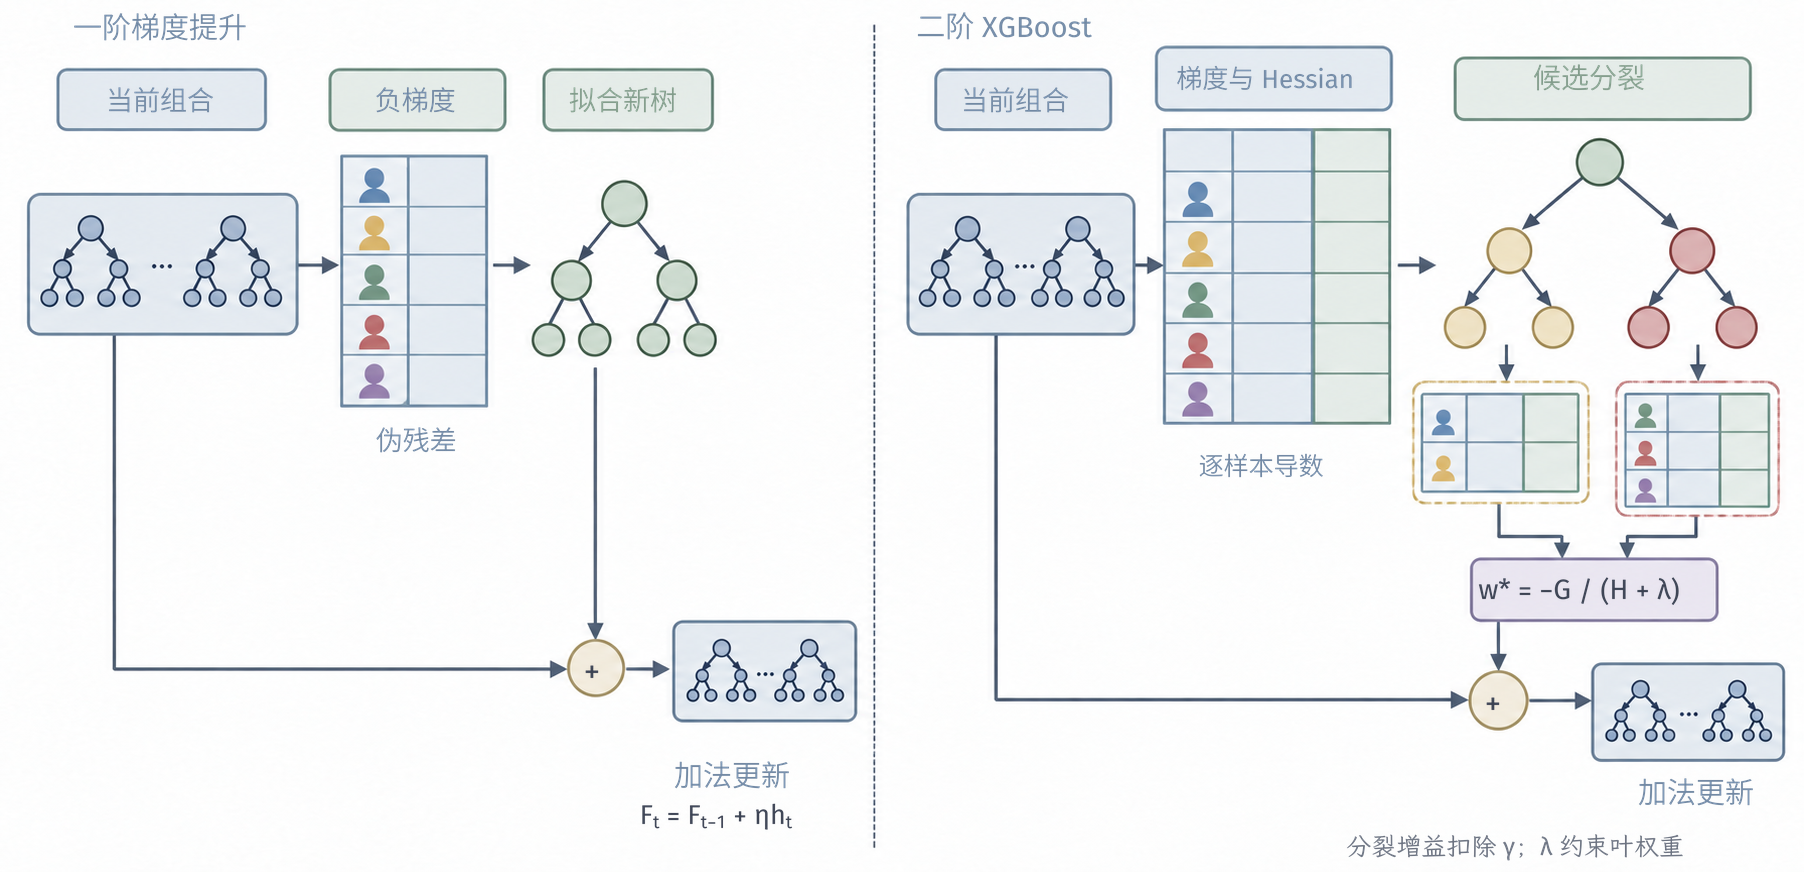
\includegraphics[width=152.739mm]{figures/07-classic-models/00-shared/generated/ensemble-gradient-xgboost/figure.png}
  \caption{梯度提升与XGBoost二阶叶目标示意（教学构造）。}
  \label{fig:ensemble-gradient-xgboost}
\end{figure*}

\subsection{LightGBM}
\label{sec:ensemble-lightgbm}

连续特征的切点随样本量线性增多，逐枚枚举统计梯度代价很高；LightGBM的预测结构仍是回归树加法，所有改动都发生在搜索与统计这一层。

\subsubsection{模型结构}
\term{LightGBM}的预测结构仍是逐轮回归树加法：本轮树划分叶区域、给出叶输出，累加到当前得分；这与前面的提升树相同。直方图、GOSS与EFB是学习过程中的计算工具，不改变预测模型本身。

\subsubsection{参数学习}

\paragraph{直方图与树的生长}
把连续特征离散为若干桶，只在桶边界上统计一阶导与曲率，形成直方图；桶内差异被忽略，桶数是精度与成本的权衡。合并父节点与一侧子节点的直方图即得另一侧，减少统计量计算。生长方式为按叶分裂（leaf-wise）：每次选增益最大的叶继续分裂，把容量投向局部收益最大处；叶数、深度与最小叶样本数共同限制失衡。

\paragraph{样本统计的GOSS近似}
\term{基于梯度的单边采样}（gradient-based one-side sampling, GOSS）按梯度大小分组：超过阈值的大梯度样本全保留，其余小梯度样本按比例$q$随机采样；被采中小梯度样本的梯度与曲率汇总按$1/q$放大，补偿未采样部分的贡献。分组阈值与采样比例$q$在验证中选择；无偏采样统计量不等于选择后无偏的比率或增益\scite{ke2017lightgbm}。

\paragraph{稀疏特征的EFB编码}
\term{互斥特征捆绑}（exclusive feature bundling, EFB）把很少同时非零的稀疏列压入同一直方图，为每个原列分配互不重叠的桶位；由桶位反查原列，非零桶计入该列的梯度曲率统计，零桶保留默认计数，候选分裂仍对应原特征。捆绑记录冲突数量与信息损失。直方图、GOSS、EFB分别改变候选阈值、样本统计与特征表示，三者在同一划分与预算下比较。

\begin{figure*}[htbp]
  \centering
  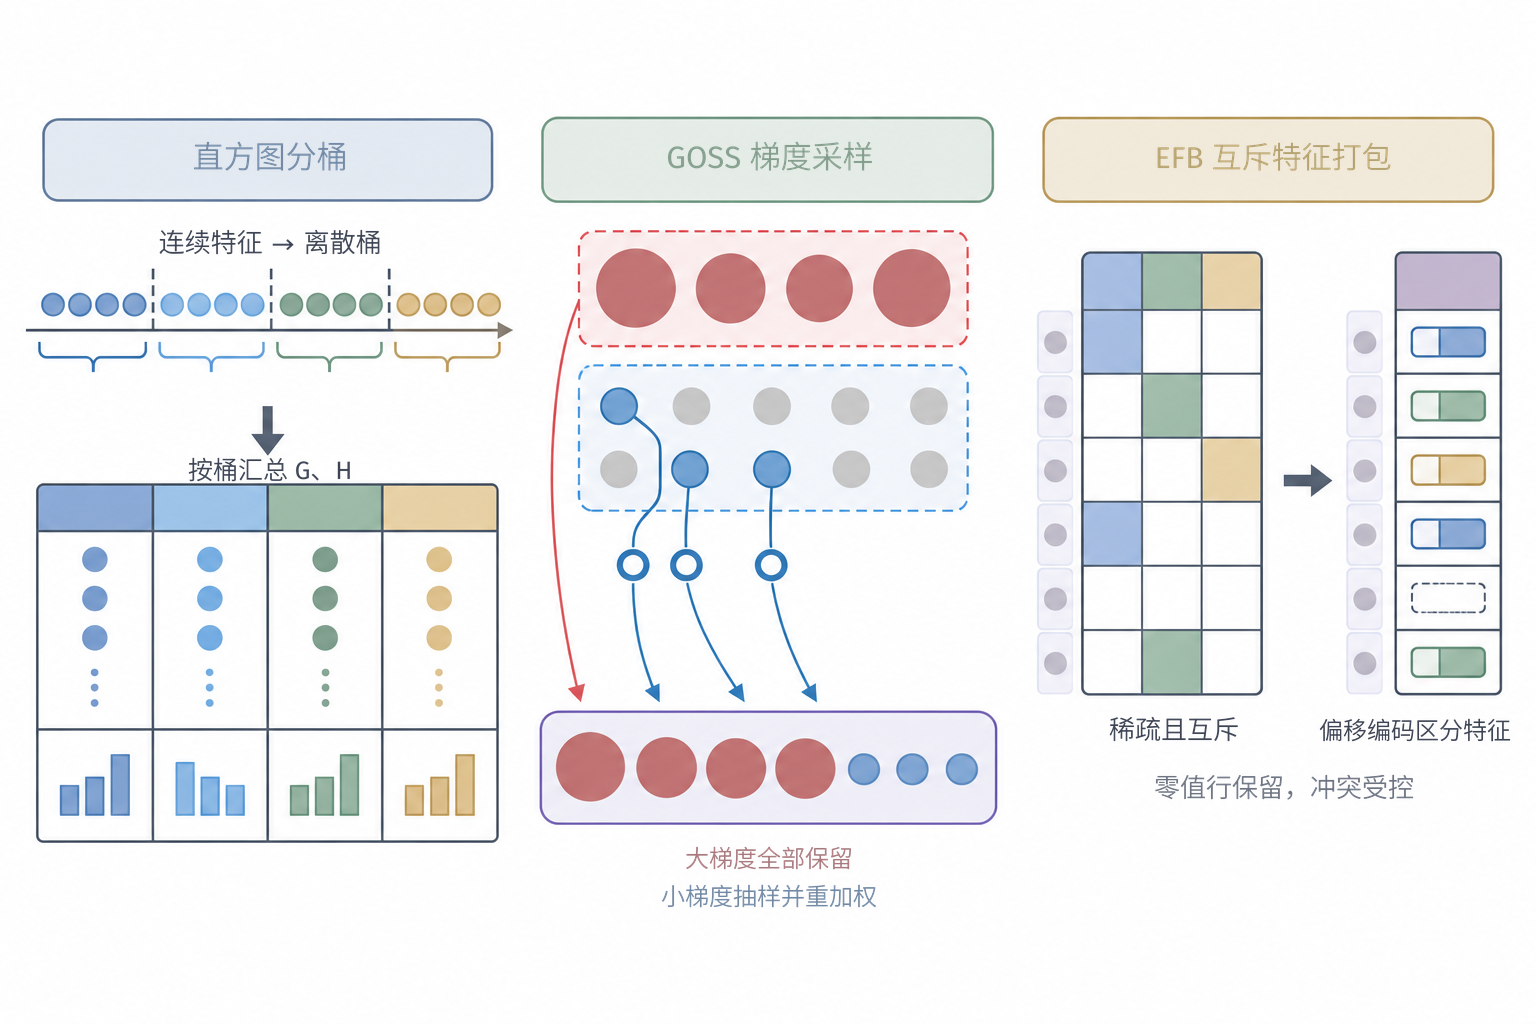
\includegraphics[width=130.048mm]{figures/07-classic-models/00-shared/generated/ensemble-lightgbm-approximations/figure.png}
  \caption{直方图、GOSS与EFB三类近似工具的作用位置示意（教学构造）。}
  \label{fig:ensemble-lightgbm-approximations}
\end{figure*}

\subsection{CatBoost}
\label{sec:ensemble-catboost}

高基数类别特征做独热编码维度爆炸，直接拿类别当前标签做编码又会偷看部署时拿不到的信息。CatBoost在树加法结构上换成用历史标签平滑得到的有序类别统计。

\subsubsection{模型结构}
\term{CatBoost}在树加法结构上增加有序类别统计：类别先由同类别历史标签平滑成数值统计量，再进入树；新输入的类别只按已观测训练记录的统计编码，不使用部署时拿不到的标签。树采用对称结构，同一层使用相同分裂条件，便于路径编码与预测，但便利不等于必然提升精度。

\subsubsection{参数学习}

\paragraph{有序类别统计}
取随机排列前缀，用前缀内同类别样本的标签统计加先验平滑作为该类别的编码：
\begin{equation}
  \hat p_c=\frac{\sum_{i\in\mathrm{prefix},\,x_i=c}y_i+\alpha p}{\#\{i\in\mathrm{prefix},\,x_i=c\}+\alpha},
  \label{eq:ensemble-catboost-codestat}
\end{equation}
先验$p$与平滑系数$\alpha$按数据来源设定，无前驱时退回先验。进入统计的是前缀内同类别标签；低频类别的不确定性由平滑系数控制。

\paragraph{有序提升}
当前预测若直接使用当前标签会造成泄漏（训练时偷看了部署时拿不到的标签信息）。\term{有序提升}（ordered boosting）让每条记录的本轮预测只由排在它之前的样本产生，修正信号也基于该前缀；理想上每条记录应有独立的训练与更新，实际通过共享树结构与状态近似，区分有序（Ordered）与普通（Plain）两种实现\scite{prokhorenkova2018catboost}。

\begin{figure*}[htbp]
  \centering
  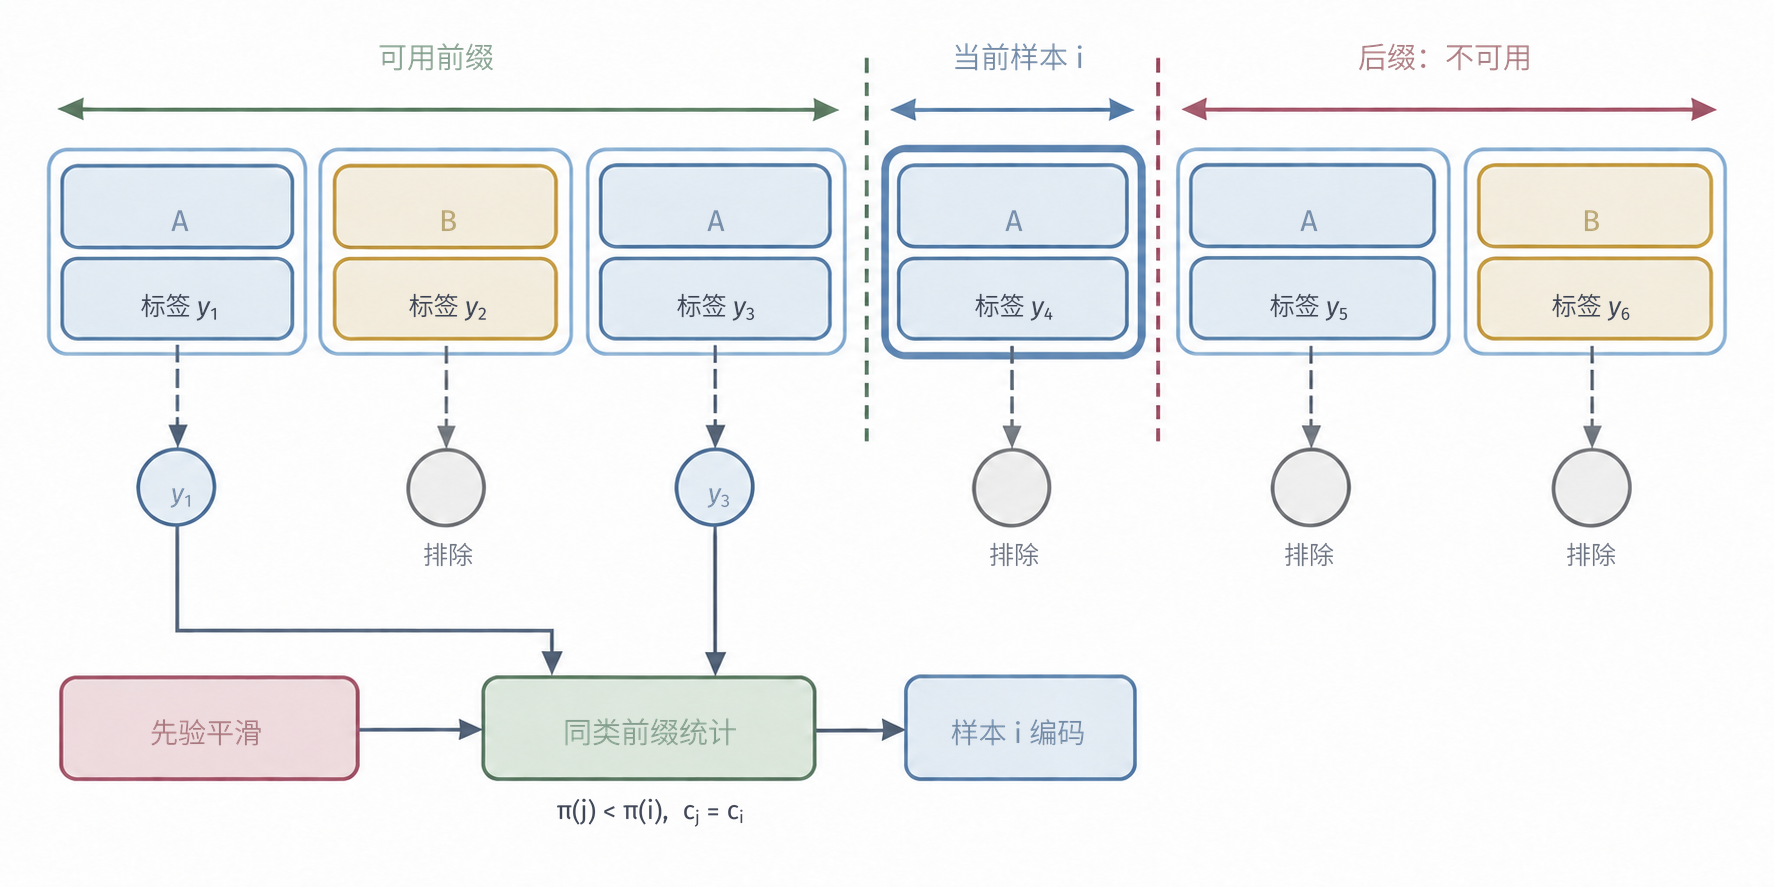
\includegraphics[width=150.199mm]{figures/07-classic-models/00-shared/generated/ensemble-catboost-ordered-statistics/figure.png}
  \caption{有序类别统计与有序提升的前缀依赖示意（教学构造）。}
  \label{fig:ensemble-catboost-ordered-statistics}
\end{figure*}

\subsection{本节比较}
\label{sec:ensemble-boosting-comparison}
各Boosting方法的修正来源不同：AdaBoost用加权错误率确定投票系数，GBDT用负梯度方向，XGBoost用二阶叶目标；候选搜索、类别编码与标签使用方式也不同。它们共享顺序加法框架，工具（直方图、GOSS、EFB、有序统计）不等于学习目标。比较时使用相同损失、数据划分、树容量与调参预算，记录训练与部署成本；轮次依赖与目标改善不保证通用优劣排序。

\begin{table}[htbp]
  \centering
  \small
  \begin{tabularx}{\linewidth}{@{}>{\RaggedRight\arraybackslash}p{20mm}>{\RaggedRight\arraybackslash}X>{\RaggedRight\arraybackslash}X>{\RaggedRight\arraybackslash}X@{}}
    \toprule
    方法 & 修正信号 & 成员族 & 特点\\
    \midrule
    AdaBoost & 加权错误率$\to$投票系数 & 二元弱成员 & 指数损失，样本重加权\\
    GBDT & 负梯度 & 叶常数回归树 & 逐叶步幅，可配收缩/随机/DART/分位数\\
    LogitBoost & 二阶工作响应 & 实数值logit修正 & 完整logit加权最小二乘\\
    XGBoost & 一阶导+曲率 & 带罚回归树 & 二阶叶值、缺失路由、计算组织\\
    LightGBM & 二阶（同XGBoost框架） & 回归树 & 直方图/GOSS/EFB工具\\
    CatBoost & 二阶（有序前缀） & 对称树 & 有序类别统计、有序提升\\
    \bottomrule
  \end{tabularx}
  \caption{Boosting各方法的修正来源与机制比较。}
  \label{tab:ensemble-boosting-comparison}
\end{table}
